\begin{savequote}[8cm]
  ``Confession: I played golf. Confession: I hired a cleaning lady. Confession: I am owner of the Turbo nose-hair trimmer with optional ear-hair accessory.''
  \qauthor{Dan Zevin}
\end{savequote}
\makeatletter
\chapter{Basics}
\label{Basics}


\section{Notational Conventions}
\label{Basics:Notation}

Every point $\V{x} \in \R^3 \setminus \set{\V{0}}$ given in Cartesian coordinates by the vector 
$\paren{x_1,x_2,x_3}^{\transp}$ can be uniquely described in spherical coordinates by a vector
$\paren{r,\vtheta,\vphi}^{\transp}$ with $r \in \Rp$, $\vtheta \in \interv{[}{0}{\pi}{]}$ and 
$\vphi \in \interv{[}{0}{2\pi}{)}$.
We have
\begin{eqnarray*}
  \paren{x_1,x_2,x_3}^{\transp} & = & \paren{r \sin \vtheta \cos \vphi, r \sin \vtheta \sin \vphi, r \cos \vtheta}^{\transp}\\
  r & = & \sqrt{x_1^2+x_2^2+x_3^2} = \norm{\V{x}}_2.
\end{eqnarray*} 
We denote by $\twosphere$ the unit sphere embedded into $\R^3$, i.e. 
$$\twosphere := \pset{\V{x} \in \R^{3}}{|}{\norm{\V{x}}_2=1}$$ 
and identify $\V{\xi} \in \twosphere$ with the vector $\paren{\vtheta,\vphi}^{\transp}$. The 
spherical coordinate system is illustrated in Figure \ref{sphere}.

Now let $\V{\xi} = \paren{\vtheta,\vphi}^{\transp}$, $\V{\eta} = \paren{\vtheta',\vphi'}^{\transp} \in
\twosphere$ and $\alpha$ be the angle spanned by the origin, $\V{\xi}$ and $\V{\eta}$.
Then the standard scalar product
$\V{\xi} \cdot \V{\eta} = \cos\left(\alpha\right)$ is given by
\begin{equation}
  \nonumber
  \fun{\cos}{\alpha} = \cos\vtheta\cos\vtheta' +
  \sin\vtheta\sin\vtheta'\fun{\cos}{\vphi-\vphi'}.
\end{equation}

The space of \emph{homogeneous polynomials} of degree $k \in \NZ$ in $\R^3$ is denoted by
$\fun{\text{Hom}_k}{\R^3}$, comprising all polynomials $Q_k \in \Pol_{n}\paren{\R}$ fulfilling 
$\fun{Q_k}{\alpha\:\V{x}} = \alpha^k \fun{Q_k}{\V{x}}$ for arbitrary $\alpha \in \R$ and $\V{x}
\in \R^3$. The proper subspace of \emph{harmonic homogeneous polynomials} of
degree $k$ is defined by
\begin{equation}
  \nonumber
  \fun{\text{Harm}_k}{\R^3} = \pset{Q_k \in \fun{\text{Hom}_k}{\R^3}}{|}{\Delta_{\V{x}} Q \equiv 0},
\end{equation}
where $\Delta_{\V{x}}$ is the Laplacian
\begin{equation}
  \nonumber
  \Delta_{\V{x}} = \frac{\partial^2}{\partial x_1^2} + \frac{\partial^2}{\partial x_2^2} +
  \frac{\partial^2}{\partial x_3^2}.
\end{equation}
Furthermore, we have
\begin{align}
  \nonumber
  \fun{\dim}{\fun{\text{Hom}_k}{\R^3}} & = \frac{(k+1)(k+2)}{2}, & 
  \fun{\dim}{\fun{\text{Harm}_k}{\R^3}} = 2k+1.
\end{align}
To keep it short we let $\Pol_{n}\paren{\twosphere} := \left.\Pol_{n}\paren{\R}\right|_{\twosphere}$ and $\mathcal{H}_k := \left.\fun{\text{Harm}_k}{\R^3}\right|_{\twosphere}$. For 
further information see for example \cite{frgesc}*{Chapters 2.3 and 2.3}.

\begin{figure}[htb]
  \centering
  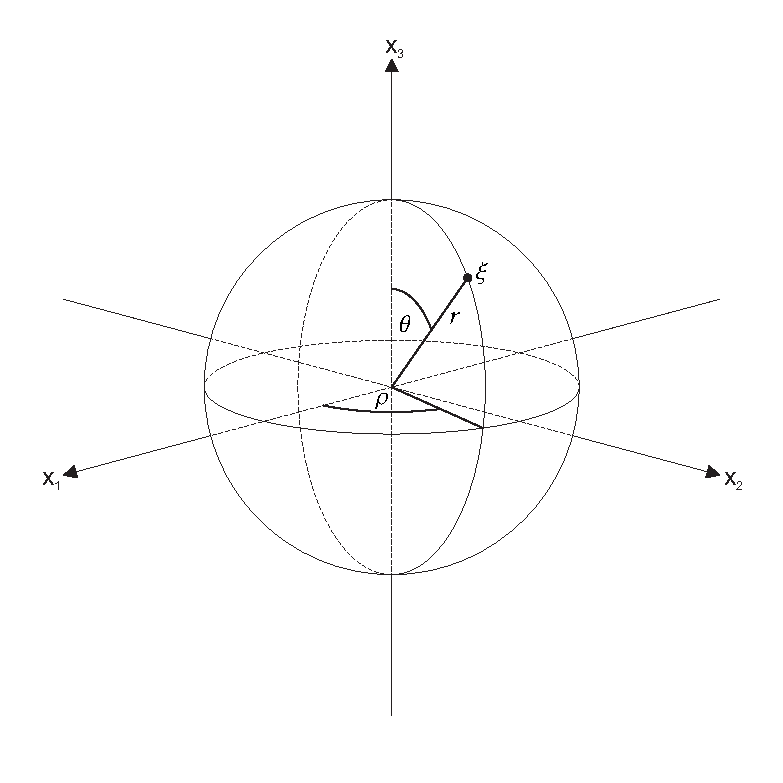
\includegraphics[height=12cm,width=12cm]{images/sphere}
  \caption{The spherical coordinate system in $\R^3$. Every point $\V{\xi}$ on a
  sphere with radius $r$ around the origin can be uniquely described by angles 
  $\vtheta$, $\vphi$ and the radius $r$. For $\vtheta = 0$ or
  $\vtheta = \pi$ the point $\V{\xi}$ coincides with the North or the South
  pole, respectively.}
  \label{sphere}
\end{figure}

\section{Legendre Functions}
\label{Basics:LegendreTypeFunctions}
In this section we briefly introduce \emph{Legendre polynomials}, \emph{associated Legendre functions} 
and \emph{associated Legendre polynomials} and collect some basic properties. These functions play 
a major role in Fourier analysis on the sphere and are key for the algorithms related to Fourier 
expansions developed in this text.

The Legendre polynomials $P_k : \interv{[}{-1}{1}{]} \rightarrow \R$, $k \in \N_{0}$ 
as classical orthogonal polynomials are given by their corresponding 
\emph{Rodrigues formula}
\begin{equation}
  \nonumber
  \fun{P_k}{x} := \frac{1}{2^k k!} \frac{\dx^k}{\dx x^k} \paren{x^2-1}^k.
\end{equation}
One verifies $\fun{P_{k}}{\pm1} = \paren{\pm1}^{k}$ and $\max_{x \in \interv{[}{-1}{1}{]}} \abs{\fun{P_{k}}{x}} = 1$ (\cite{niuv}*{pp. 4\ndash47}).
%The corresponding three-term recurrence relation is
%\begin{equation}
%  \nonumber
%  \paren{k+1}\fun{P_{k+1}}{x} = \paren{2k+1}x\fun{P_{k}}{x} -
%  k\fun{P_{k-1}}{x},\ k \in \N.
%\end{equation}
Furthermore we define the associated Legendre functions $P_k^n : \interv{[}{-1}{1}{]} \rightarrow \R$ by
\begin{equation}
  \nonumber
  \fun{P_k^n}{x} := \sqrt{\frac{\paren{k-n}!}{\paren{k+n}!}}
  \paren{1-x^2}^{n/2} \frac{\dx^n}{\dx x^n} \fun{P_k}{x} \quad \paren{n \in \NZ,\ k=n,n+1,\ldots}.
\end{equation}
For fixed $n$ the set $\set{P_{k}^n}_{k=n,n+1,\ldots}$ form a complete set of orthogonal functions 
for $\Ln{2}{\interv{[}{-1}{1}{]}}$ with
$$ \scalarproduct{P_{k}^n}{P_{l}^n}_{\interv{[}{-1}{1}{]}} = \int_{-1}^{1} \fun{P_{k}^n}{x} \fun{P_{l}^n}{x} \dx x = \frac{2}{2k+1} \delta_{k,l} \quad \paren{0 \le n \le k,l}.$$
The associated Legendre functions fulfill the three-term recurrence
\begin{equation}
  \label{Basics:AssociatedLegendreDefinition}
  \begin{split}
    \fun{P_{n-1}^n}{x} & = 0,\qquad \fun{P_{n}^n}{x} = \frac{((2n)!)}{2^n n!}^{1/2} \paren{1-x^2}^{n/2},\\
    \fun{P_{k+1}^n}{x} & = v_{k}^n x \fun{P_{k}^n}{x} + w_{k}^n \fun{P_{k-1}^n}{x} \quad (k = n,n+1,\ldots),
  \end{split}
\end{equation}
where
\begin{equation} 
  \label{Basics:AssociatedLegendreRecurrenceCoefficients}
v_{k}^n := \frac{2k+1}{((k-n+1)(k+n+1))^{1/2}}\; ,\qquad w_{k}^n := - \frac{((k-n)(k+n))^{1/2}}{((k-n+1)(k+n+1))^{1/2}}.
\end{equation}
A simple but at the same time very important idea is to define the associated Legendre functions $P_k^n$ also for 
$k < n$ by means of the modified three-term recurrence
\begin{equation} 
  \label{Basics:AssociatedLegendreDefinitionExtended}
  \fun{P_{k+1}^n}{x} = \paren{\alpha_{k}^n x + \beta_{k}^n} \fun{P_{k}^n}{x} + \gamma_{k}^n \fun{P_{k-1}^n}{x}\quad\paren{k \in \NZ}
\end{equation}
with
\begin{eqnarray*}
  \alpha_{k}^n & := & \left\{
    \begin{array}{ll}
      (-1)^{k+1} & \text{for}\ k < n,\\
      v_{k}^n    & \text{otherwise},
    \end{array}\right.\\
  \beta_{k}^n & := & \left\{
    \begin{array}{lll}
      1 & \text{for}\ k < n,\\
      0 & \text{otherwise},
    \end{array}\right.\\
  \gamma_{k}^n & := & \left\{
    \begin{array}{lll}
      0       & \text{for}\ k \leq n,\\
      w_{k}^n & \text{otherwise.}
    \end{array}\right.\\
\end{eqnarray*}
For even $n$ we let
$$ \fun{P_{-1}^n}{x} := 0,\ \fun{P_{0}^n}{x} := \sqrt{\frac{(2n)!}{2^n n!}}$$
and for odd $n$ we start with
$$ \fun{P_{0}^n}{x} := \fun{P_{1}^n}{x} := \sqrt{\frac{(2n)!}{2^n n!}} \paren{1-x^2}^{1/2}.$$
For $k \ge n$ this definition coincides with \eqref{Basics:AssociatedLegendreDefinition}. 
As a matter of fact, $P_{k}^n$ is a polynomial of degree $k$ for even $n$ while 
$\paren{1-x^2}^{-1/2}P_{k}^n$ is a polynomial of degree $k-1$ for odd $n$.

Based on the recurrence coefficients from \eqref{Basics:AssociatedLegendreRecurrenceCoefficients} 
and introducing a shift parameter $c \in \NZ$, we 
define the associated Legendre polynomials $\fun{P_{k}^n}{\cdot,c}$ by
\begin{equation}
  \label{Basics:AssociatedLegendrePolynomials}
  \begin{split}
    & \fun{P_{-1}^n}{x,c} := 0,\ \fun{P_{0}^n}{x,c} := 1,\\
    & \fun{P_{k+1}^n}{x,c} = \paren{\alpha_{k+c}^n x + \beta_{k+c}^n} \fun{P_{k}^n}{x,c} + \gamma_{k+c}^n \fun{P_{k-1}^n}{x,c}.
  \end{split}
\end{equation}
Now straightforward induction yields
\begin{lemma}
  \label{Basics:AssociatedLegendreRecurrence}
  Let the functions $P_{k}^n$ and $\fun{P_{k}^n}{\cdot,c}$ be given as in \eqref{Basics:AssociatedLegendreDefinitionExtended} and 
  \eqref{Basics:AssociatedLegendrePolynomials}. Then we have
  $$ \fun{P_{c+k}^n}{x} = \fun{P_{k}^n}{x,c} \fun{P_{c}^n}{x} + \gamma_{c}^n \fun{P_{k-1}^n}{x,c+1} \fun{P_{c-1}^n}{x}. $$
\end{lemma}

\section{Spherical Harmonics}
\label{Basics:SphericalHarmonics}

\emph{Spherical harmonics} on the sphere $\twosphere$ arise the same way as complex exponentials 
$\e^{\im k x}$ on the Torus $\mathbb{T}$ and form a complete orthogonal system for $\Ln{2}{\twosphere}$.
Speaking of Fourier analysis with respect to the sphere, one refers to spherical harmonics as the Fourier 
basis on $\twosphere$. 
%In this section, we shortly introduce these basis functions mentioning basic properties.

From Laplace's differential equation $\Delta f = 0$ in $\R^3$, one obtains in spherical coordinates
\begin{equation}
  \label{Basics:LaplaceBeltrami}
  \Delta f = \frac{\partial^2 f}{\partial r^2} + \frac{2}{r}\frac{\partial f}{\partial
  r} + \frac{1}{r^2 \sin \vtheta}\frac{\partial}{\partial \vtheta}\paren{\sin \vtheta \: \frac{\partial f}{\partial
  \vtheta}} + \frac{1}{r^2 \sin \vtheta}\frac{\partial^2}{\partial \vphi^2} = 0.
\end{equation}
%*** \begin{comment}Add reference here\end{comment}
Using an ansatz based on separation of variables (see \cite{co2}) and taking into account that $r = 1$ when restricting 
\eqref{Basics:LaplaceBeltrami} to $\twosphere$, one obtains the solutions
\begin{equation}
  \label{Basics:SphericalHarmonicsDefinition}
  \begin{split}
    & Y_{k}^n: \twosphere \rightarrow \C \quad \paren{n \in \NZ,\; k = -n,-n+1,\ldots,n},\\
    & \fun{Y_{k}^n}{\vtheta,\vphi} := \sqrt{\frac{2n+1}{4\pi}} 
    \fun{P_{k}^{\abs{n}}}{\cos \vtheta} \e^{\im n \vphi}.
  \end{split}
\end{equation}
The index $k$ is called the \emph{degree} and $n$ is the \emph{order} of $Y_{k}^n$. 
Figure \ref{Basics:Figure:SphericalHarmonics} shows the absolute value of the first
functions $Y_{k}^{n}$.
Due to the separability one proves easily that they fulfill the orthogonality condition
\begin{equation}
  \nonumber
  \scalarproduct{Y_{k}^n}{Y_{l}^m}_{\twosphere} = \delta_{k,l} \delta_{n,m}
\end{equation}
with respect to the $\Ln{2}{\twosphere}$-scalar product 
\begin{equation}
  \nonumber
  \scalarproduct{Y_{k}^n}{Y_{l}^m}_{\twosphere} := \int_{0}^{2\pi} \int_{0}^{\pi} \fun{Y_{k}^n}{\vtheta,\vphi} \overline{\fun{Y_{l}^m}{\vtheta,\vphi}} \sin \vtheta \; \dx \vtheta \; \dx \vphi.
\end{equation}
An important result is that these functions all are contained in 
$\mathcal{H}_k$ so that for fixed $k \in \NZ$, the set
\begin{equation}
  \nonumber
  \pset{Y_{k}^n}{|}{n = -k,-k+1,\ldots,k}
\end{equation}
forms an orthonormal basis of $ \mathcal{H}_k$, since $\dim \mathcal{H}_k =
2k+1$. Moreover, the spaces $\mathcal{H}_k$ are orthogonal
to each other and
$$\pset{Y_{k}^n}{|}{k = 0,1,\ldots,M,\ n = -k,-k+1,\ldots,k},\ M \in \NZ$$ 
provides an orthonormal basis for the space $\bigoplus_{k=0}^{M}\mathcal{H}_k$ called
the space of \emph{spherical harmonics} of degree $M$.

At first glance, the restriction to homogeneous and harmonic polynomials
might exclude various functions from $\fun{\Pol_M}{\twosphere}$. But as a 
matter of fact these spaces are identical (see \cite{frgesc}*{Corollary 2.2.5}), i.e. 
\begin{equation}
  \nonumber
    \fun{\Pol_M}{\twosphere} = \bigoplus_{k=0}^{M}\mathcal{H}_k.
\end{equation}

\begin{figure}[htbp]
  \centering
   \subfigure[$\Re \: Y_{0}^{0}$]
     {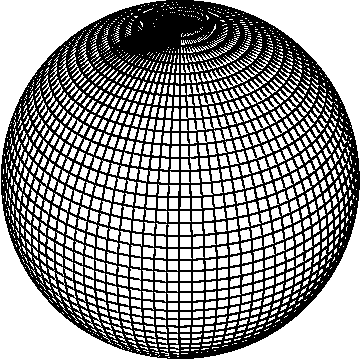
\includegraphics[width=0.5\textwidth]{images/sh_r_0_0}}\hfill
   \subfigure[$\Re \: Y_{4}^{2}$]
     {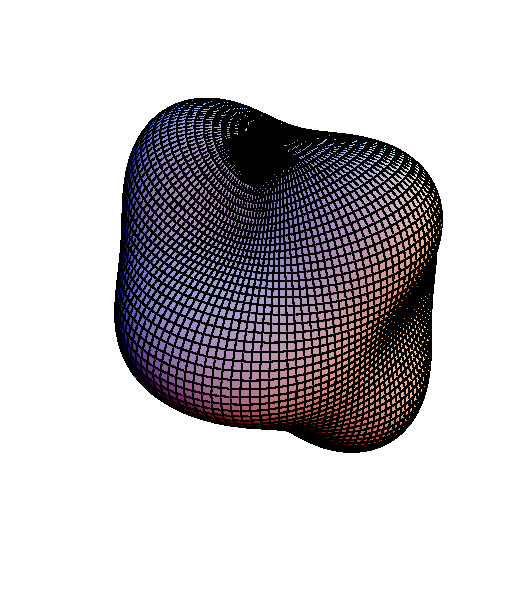
\includegraphics[width=0.5\textwidth]{images/sh_r_4_2}}\\
   \subfigure[$\Re \: Y_{9}^{5}$]
     {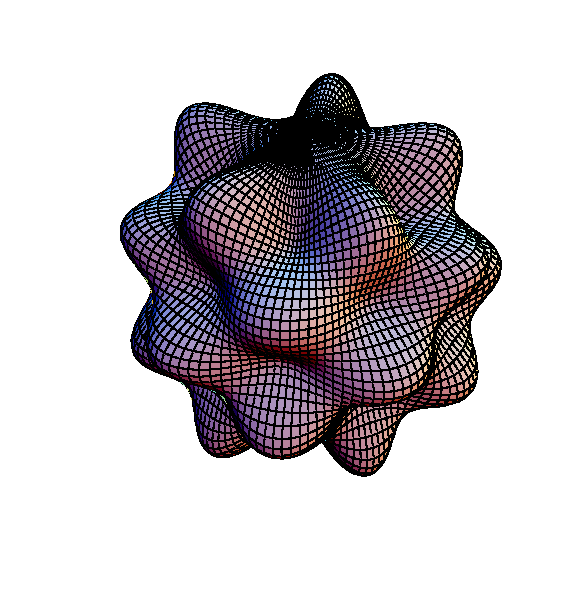
\includegraphics[width=0.5\textwidth]{images/sh_r_9_5}}\hfill
   \subfigure[$\Re \: Y_{13}^{1}$]
     {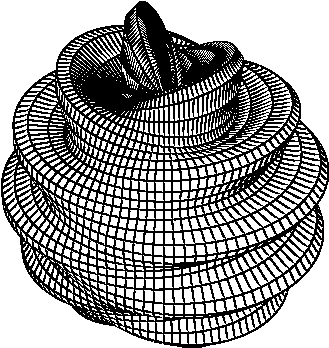
\includegraphics[width=0.5\textwidth]{images/sh_r_13_1}}\\
   \subfigure[$\Re \: Y_{13}^{6}$]
     {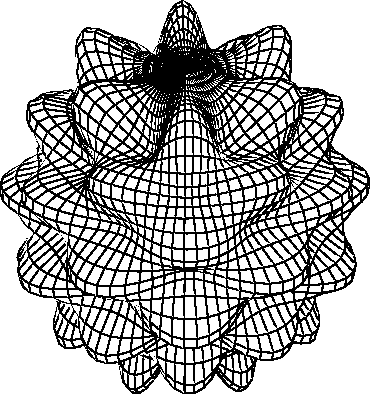
\includegraphics[width=0.5\textwidth]{images/sh_r_13_6}}\hfill
   \subfigure[$\Re \: Y_{13}^{13}$]
     {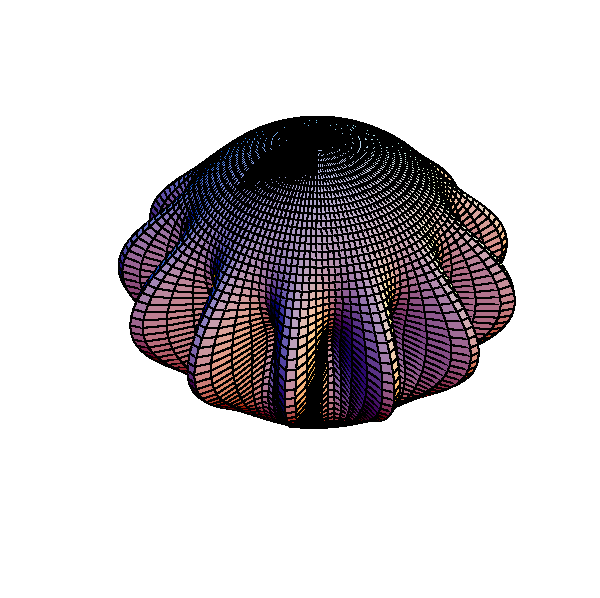
\includegraphics[width=0.5\textwidth]{images/sh_r_13_13}}\\
  \caption{The functions $\R \: Y_{k}^{n}$ for different $\paren{k,n}$.}
  \label{Basics:Figure:SphericalHarmonics}
\end{figure}

We finally mention the well known addition theorem for spherical harmonics 
that relates any set of functions $\set{H_k^n}_{n=-k}^k$ forming an orthonormal basis of $\mathcal{H}_k$ 
to the Legendre polynomial $P_{k}$.

\begin{proposition}[Addition Theorem]
  \label{Basics:AdditionTheorem}
  For every $\Ln{2}{\twosphere}$-orthonormal basis 
  $\set{H_{k}^n}_{n=-k}^{k}$ of $\mathcal{H}_k$, we have
  \begin{equation}
    \nonumber
    \sum_{n=-k}^{k} \fun{H_{k}^n}{\V{\xi}} \overline{\fun{H_{k}^n}{\V{\eta}}} =
    \frac{2k+1}{4\pi}\fun{P_k}{\V{\xi} \: \V{\eta}}.
  \end{equation}
\end{proposition}

See \cite{frgesc}*{p. 37} or \cite{co}*{pp. 172, Theorem 5} for a proof. In particular it holds for the basis functions $Y_{k}^n$ given in 
\eqref{Basics:SphericalHarmonicsDefinition}.

\section{Spherical Radial Basis Functions}
\emph{Spherical radial basis basis functions} are the spherical counterpart of radial basis functions in Euclidean spaces. 
Generally, one starts with a function $G$ from $\Ln{2}{\interv{[}{-1}{1}{]}}$
%$: \interv{[}{-1}{1}{]} \rightarrow \C$ 
and defines for fixed $\V{\eta} \in \twosphere$ the $\V{\eta}$-zonal function $K_{\V{\eta}}: \twosphere \rightarrow \C$ by
$$ \fun{K_{\V{\eta}}}{\V{\xi}} := \fun{G}{\V{\eta} \cdot \V{\xi}}.$$
By means of the \emph{Funk-Hecke formula} (see \cite[pp. 60]{frgesc}) we obtain for fixed $k \in \NZ$
$$
  \scalarproduct{G}{Y_{k}^n} = \int_{\twosphere} \fun{G}{\V{\eta} \cdot \V{\xi}} \overline{\fun{Y_{k}^n}{\V{\xi}}} \dx \V{\xi} = \fun{G^{\wedge}}{k} \overline{\fun{Y_{k}^n}{\V{\eta}}} \quad \paren{n=-k,\ldots,k},
$$
where the \emph{Legendre transform}, i.e. the \emph{symbol} of $G$, is given by
$$
  \fun{G^{\wedge}}{k} := 2 \pi \int_{-1}^{1} \fun{G}{x} \fun{P_{k}}{x} \dx x \quad \paren{k \in \NZ}.
$$
%We refer the interested reader to \cite{} and \cite{} for more details.
%The function $G$ can be developed into a series of Legendre polynomials
%$$ \fun{G}{x} = \sum_{k = 0}^{\infty} a_k \fun{P_k}{x}.$$
%where the coefficients $a_k$ are the scalar products
%$$ a_k = \scalarproduct{G}{P_{k}}_{\interv{[}{-1}{1}{]}} = \int_{-1}^{1} \fun{G}{x} \fun{P_k}{x} \dx x.$$
We have therefore 
$$
  \fun{K_{\V{\eta}}}{\V{\xi}} = \sum_{k = 0}^{\infty} \sum_{n=-k}^k \fun{G^{\wedge}}{k} \overline{\fun{Y_{k}^n}{\V{\eta}}} \fun{Y_{k}^n}{\V{\xi}} 
$$
and applying the Addition Theorem from Proposition \ref{Basics:AdditionTheorem}, we obtain the orthogonal expansion
$$
  \fun{K_{\V{\eta}}}{\V{\xi}} = \sum_{k = 0}^{\infty} \frac{2n+1}{4\pi} \fun{G^{\wedge}}{k} \fun{P_k}{\V{\eta} \cdot \V{\xi}}.
$$
%One is often interested in evaluating such an expansion on the sphere in a fast way when dealing with 
%spherical convolution. As an application of the algorithms developed in this text, one can derive 
%an algorithm based on the discrete spherical Fourier transform, as shown in Chapter \ref{}.

\begin{example}
We consider the generating series
\begin{equation}
  \label{Basics:GeneratingFunction}
  \fun{\phi}{h} := \sum_{k = 0}^{\infty} h^k \fun{P_k}{x} \quad \paren{x \in \interv{[}{-1}{1}{]}}
\end{equation}
which is absolutely and uniformly convergent for $h \in
\interv{(}{-1}{1}{)}$ with
\begin{equation}
  \label{Basics:Solution}
  \sum_{k = 0}^{\infty} h^k \fun{P_k}{x} = \frac{1}{\sqrt{1-2hx+h^2}}.
\end{equation}
This follows from the ordinary differential equation
\begin{equation}
\label{Basics:DifferentialEquation}
  \paren{1+h^2-2hx}\fun{\phi'}{h} = \paren{x-h}\fun{\phi}{h}
\end{equation}
obtained by differentiation with respect to $h$ and comparing coefficients in line with \eqref{Basics:GeneratingFunction}. Using the initial 
condition $\fun{\phi}{0}=1$ this yields the unique solution \eqref{Basics:Solution} of \eqref{Basics:DifferentialEquation}.
From this result, the identity
\begin{equation}
  \nonumber
  \sum_{k=0}^{\infty} \paren{2k+1} h^k \fun{P_k}{x} =
  \frac{1-h^2}{\paren{1-2hx+h^2}^{3/2}}
\end{equation}
 follows easily. When $h$ is restricted to $\interv{(}{0}{1}{)}$ and for fixed $\V{\eta} \in \twosphere$ the spherical radial basis function
$Q_h:\twosphere \rightarrow \R$, with
\begin{equation}
  \label{PoissonKernel}
  \nonumber
  \fun{Q_h}{\V{\eta} \cdot \V{\xi}} := \frac{1}{4\pi} \frac{1-h^2}{\paren{1-2\V{\eta} \cdot \V{\xi}+h^2}^{3/2}},
\end{equation}
is called \emph{Poisson kernel}. The symbol $\fun{Q_{h}^{\wedge}}{k}$ is given by 
$$
  \fun{Q_{h}^{\wedge}}{k} = h^k.
$$
We refer to Figures \ref{Basics:Figure:PoissonKernel} and \ref{Basics:Figure:PoissonKernel2}
for a visual impression and mention that the parameter $h$
allows for controlling the concentration of the function's energy around
$x = 1$. The Poisson kernel is a positive function and normalized with
$$
  \int_{\twosphere} \fun{Q_{h}}{\V{\xi} \cdot \V{\eta}} \dx \V{\xi} = 1.
$$
Further properties with respect to localization and smoothness are derived in \cite[pp. 112]{frgesc}.
\end{example}

\begin{example}
  The \emph{Gauss-Weierstra� kernel} $W_{\rho}: \twosphere \rightarrow \R$ is defined by
  $$
    \fun{W_{\rho}}{\V{\xi} \cdot \V{\eta}} := \sum_{k=0}^{\infty} \e^{-k(k+1)\rho} \frac{2k+1}{4\pi} \fun{P_{k}}{\V{\xi} \cdot \V{\eta}}.
  $$
  Results due to Bochner (1950, 1954) assure $\fun{W_{\rho}}{x} \ge 0$ and we have
  $$
    \int_{\twosphere} \fun{W_{\rho}}{\V{\xi} \cdot \V{\eta}} \dx \V{\xi} = 1.
  $$
  For further properties we refer to \cite{frgesc} again. The kernel function $W_{\rho}$ is illustrated in Figure \ref{Basics:Figure:PoissonKernel}.
\end{example}

\begin{figure}[tb]
  \centering
  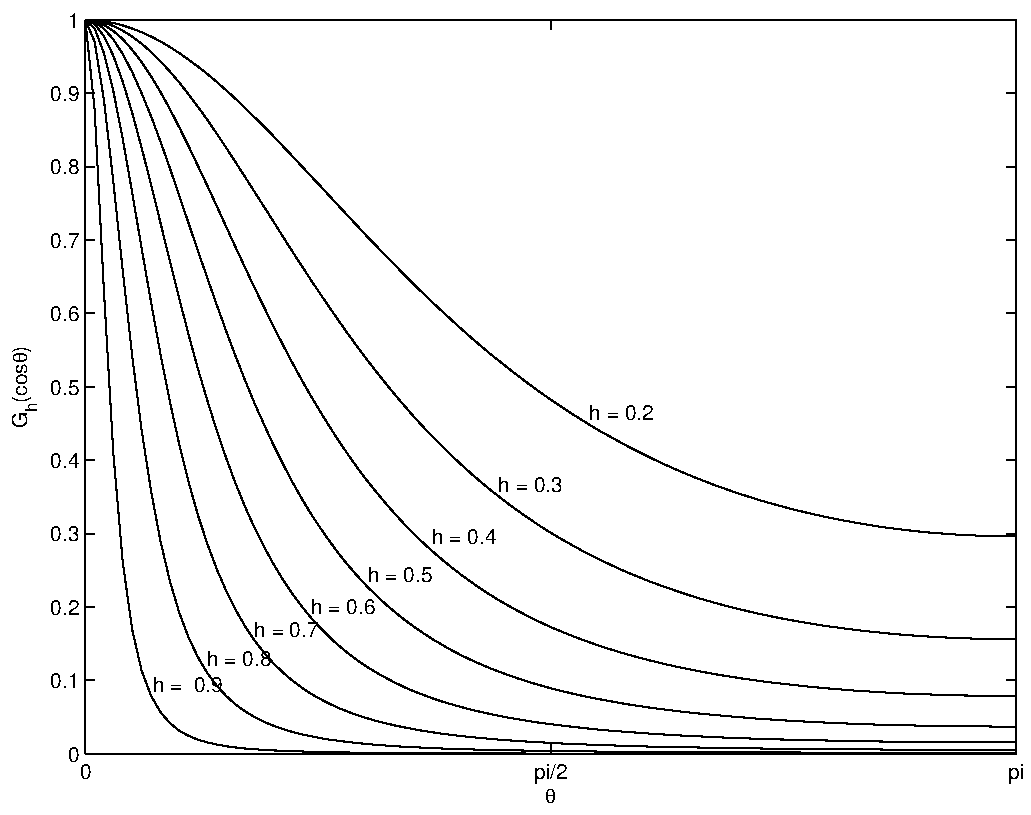
\includegraphics[width=12cm]{images/poisson}
  \caption{The Poisson kernel $\fun{Q_{h}}{\cos\theta}$ for $h = 0.5,0.6,0.7,0.8$ and $\theta \in \interv{[}{-\pi}{\pi}{]}$.}
  \label{Basics:Figure:PoissonKernel}
\end{figure}

\begin{figure}[tb]
  \centering
   \subfigure[$h=0.70$]
     {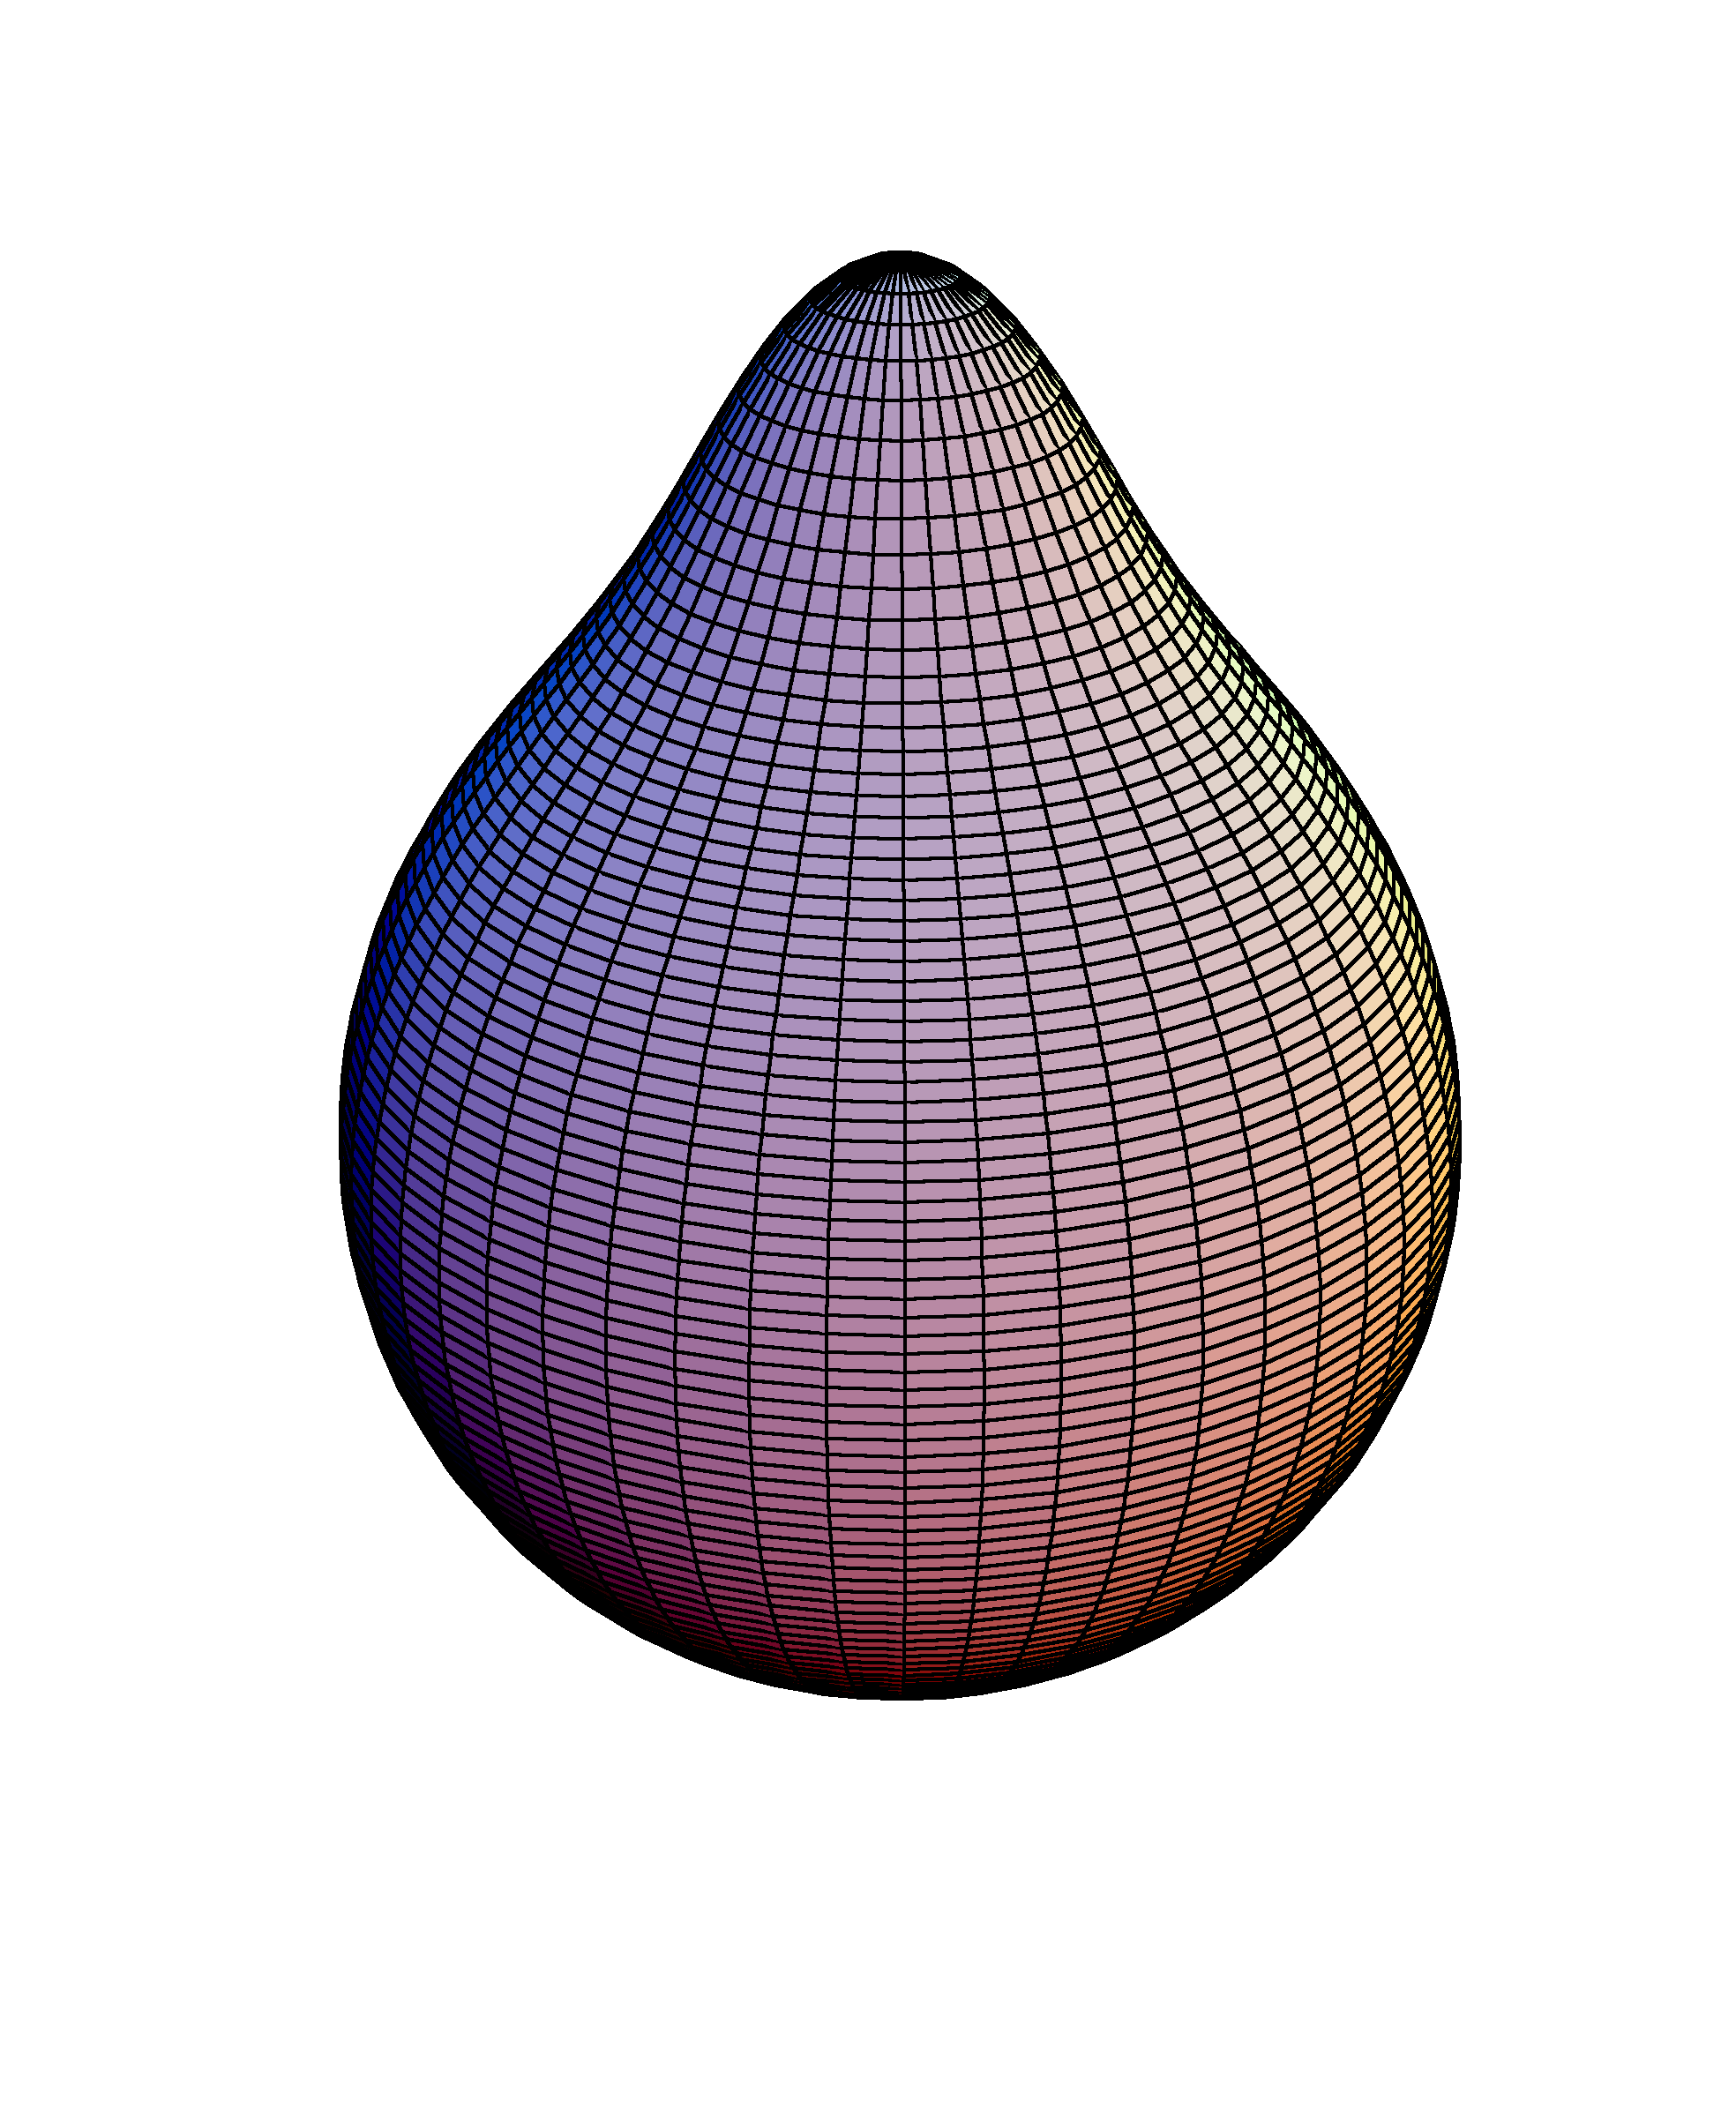
\includegraphics[width=0.5\textwidth]{images/p_070.png}}\hfill
   \subfigure[$h=0.75$]
     {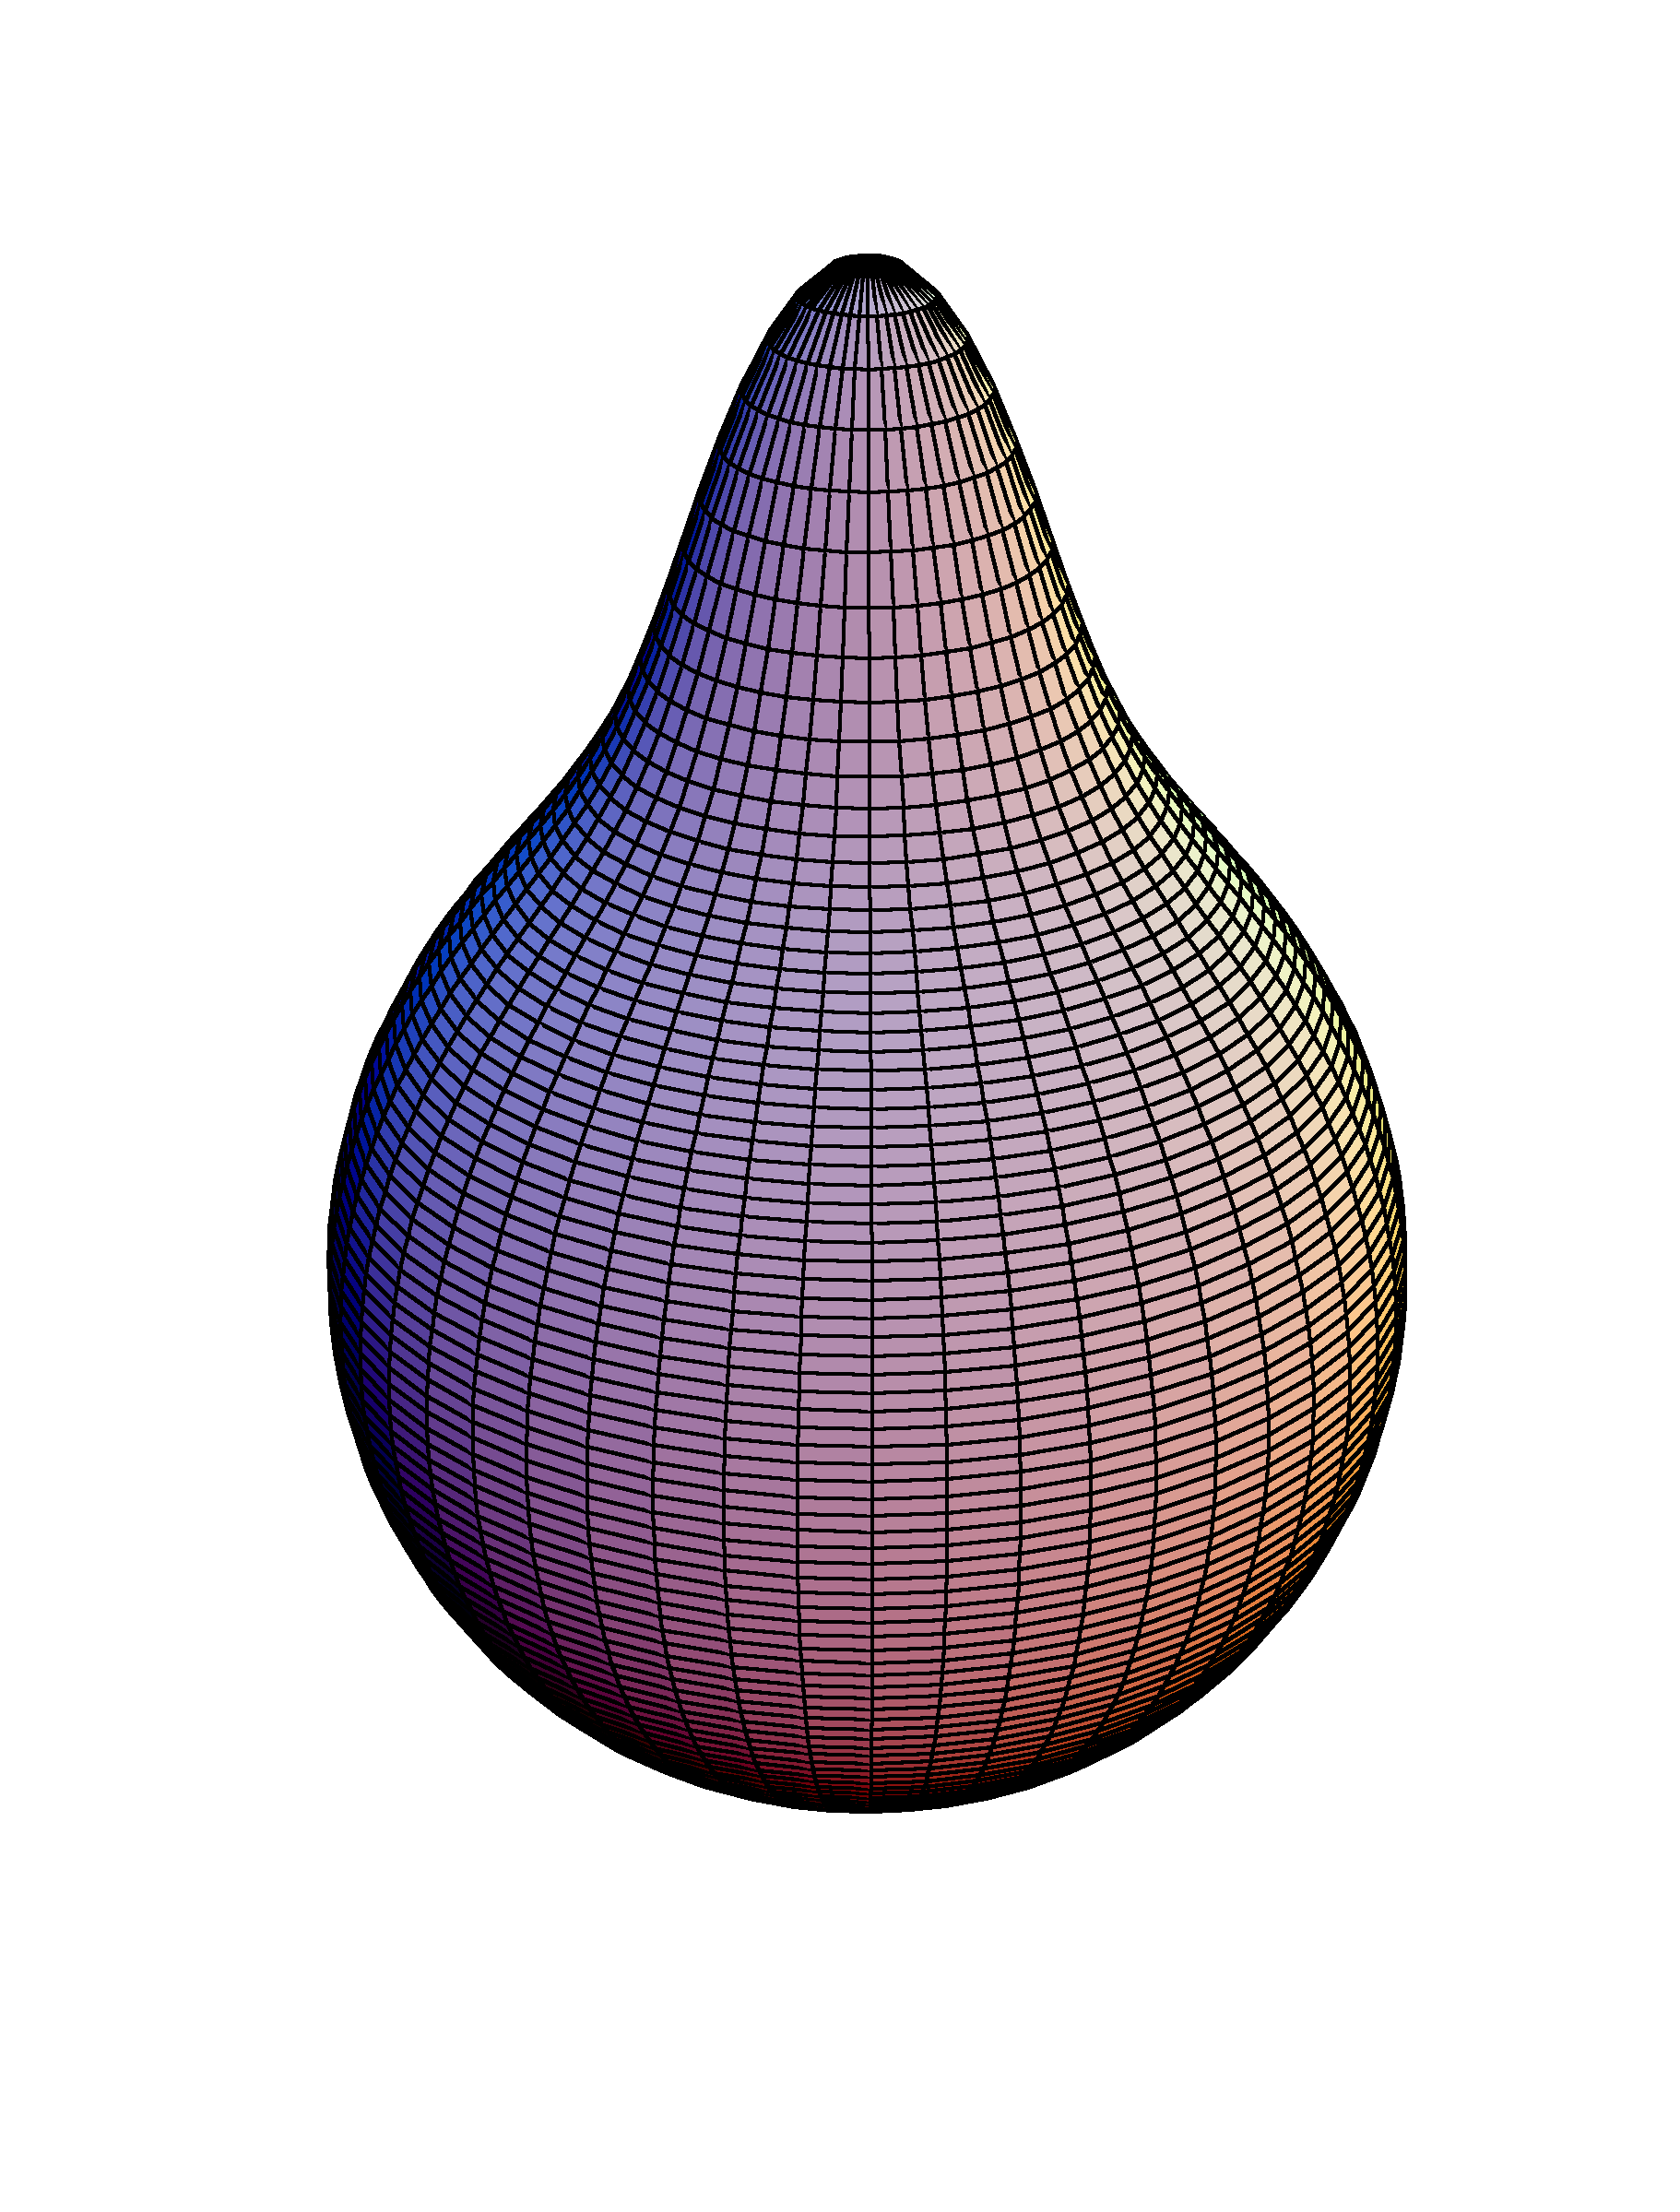
\includegraphics[width=0.5\textwidth]{images/p_075.png}}\\
   \subfigure[$h=0.80$]
     {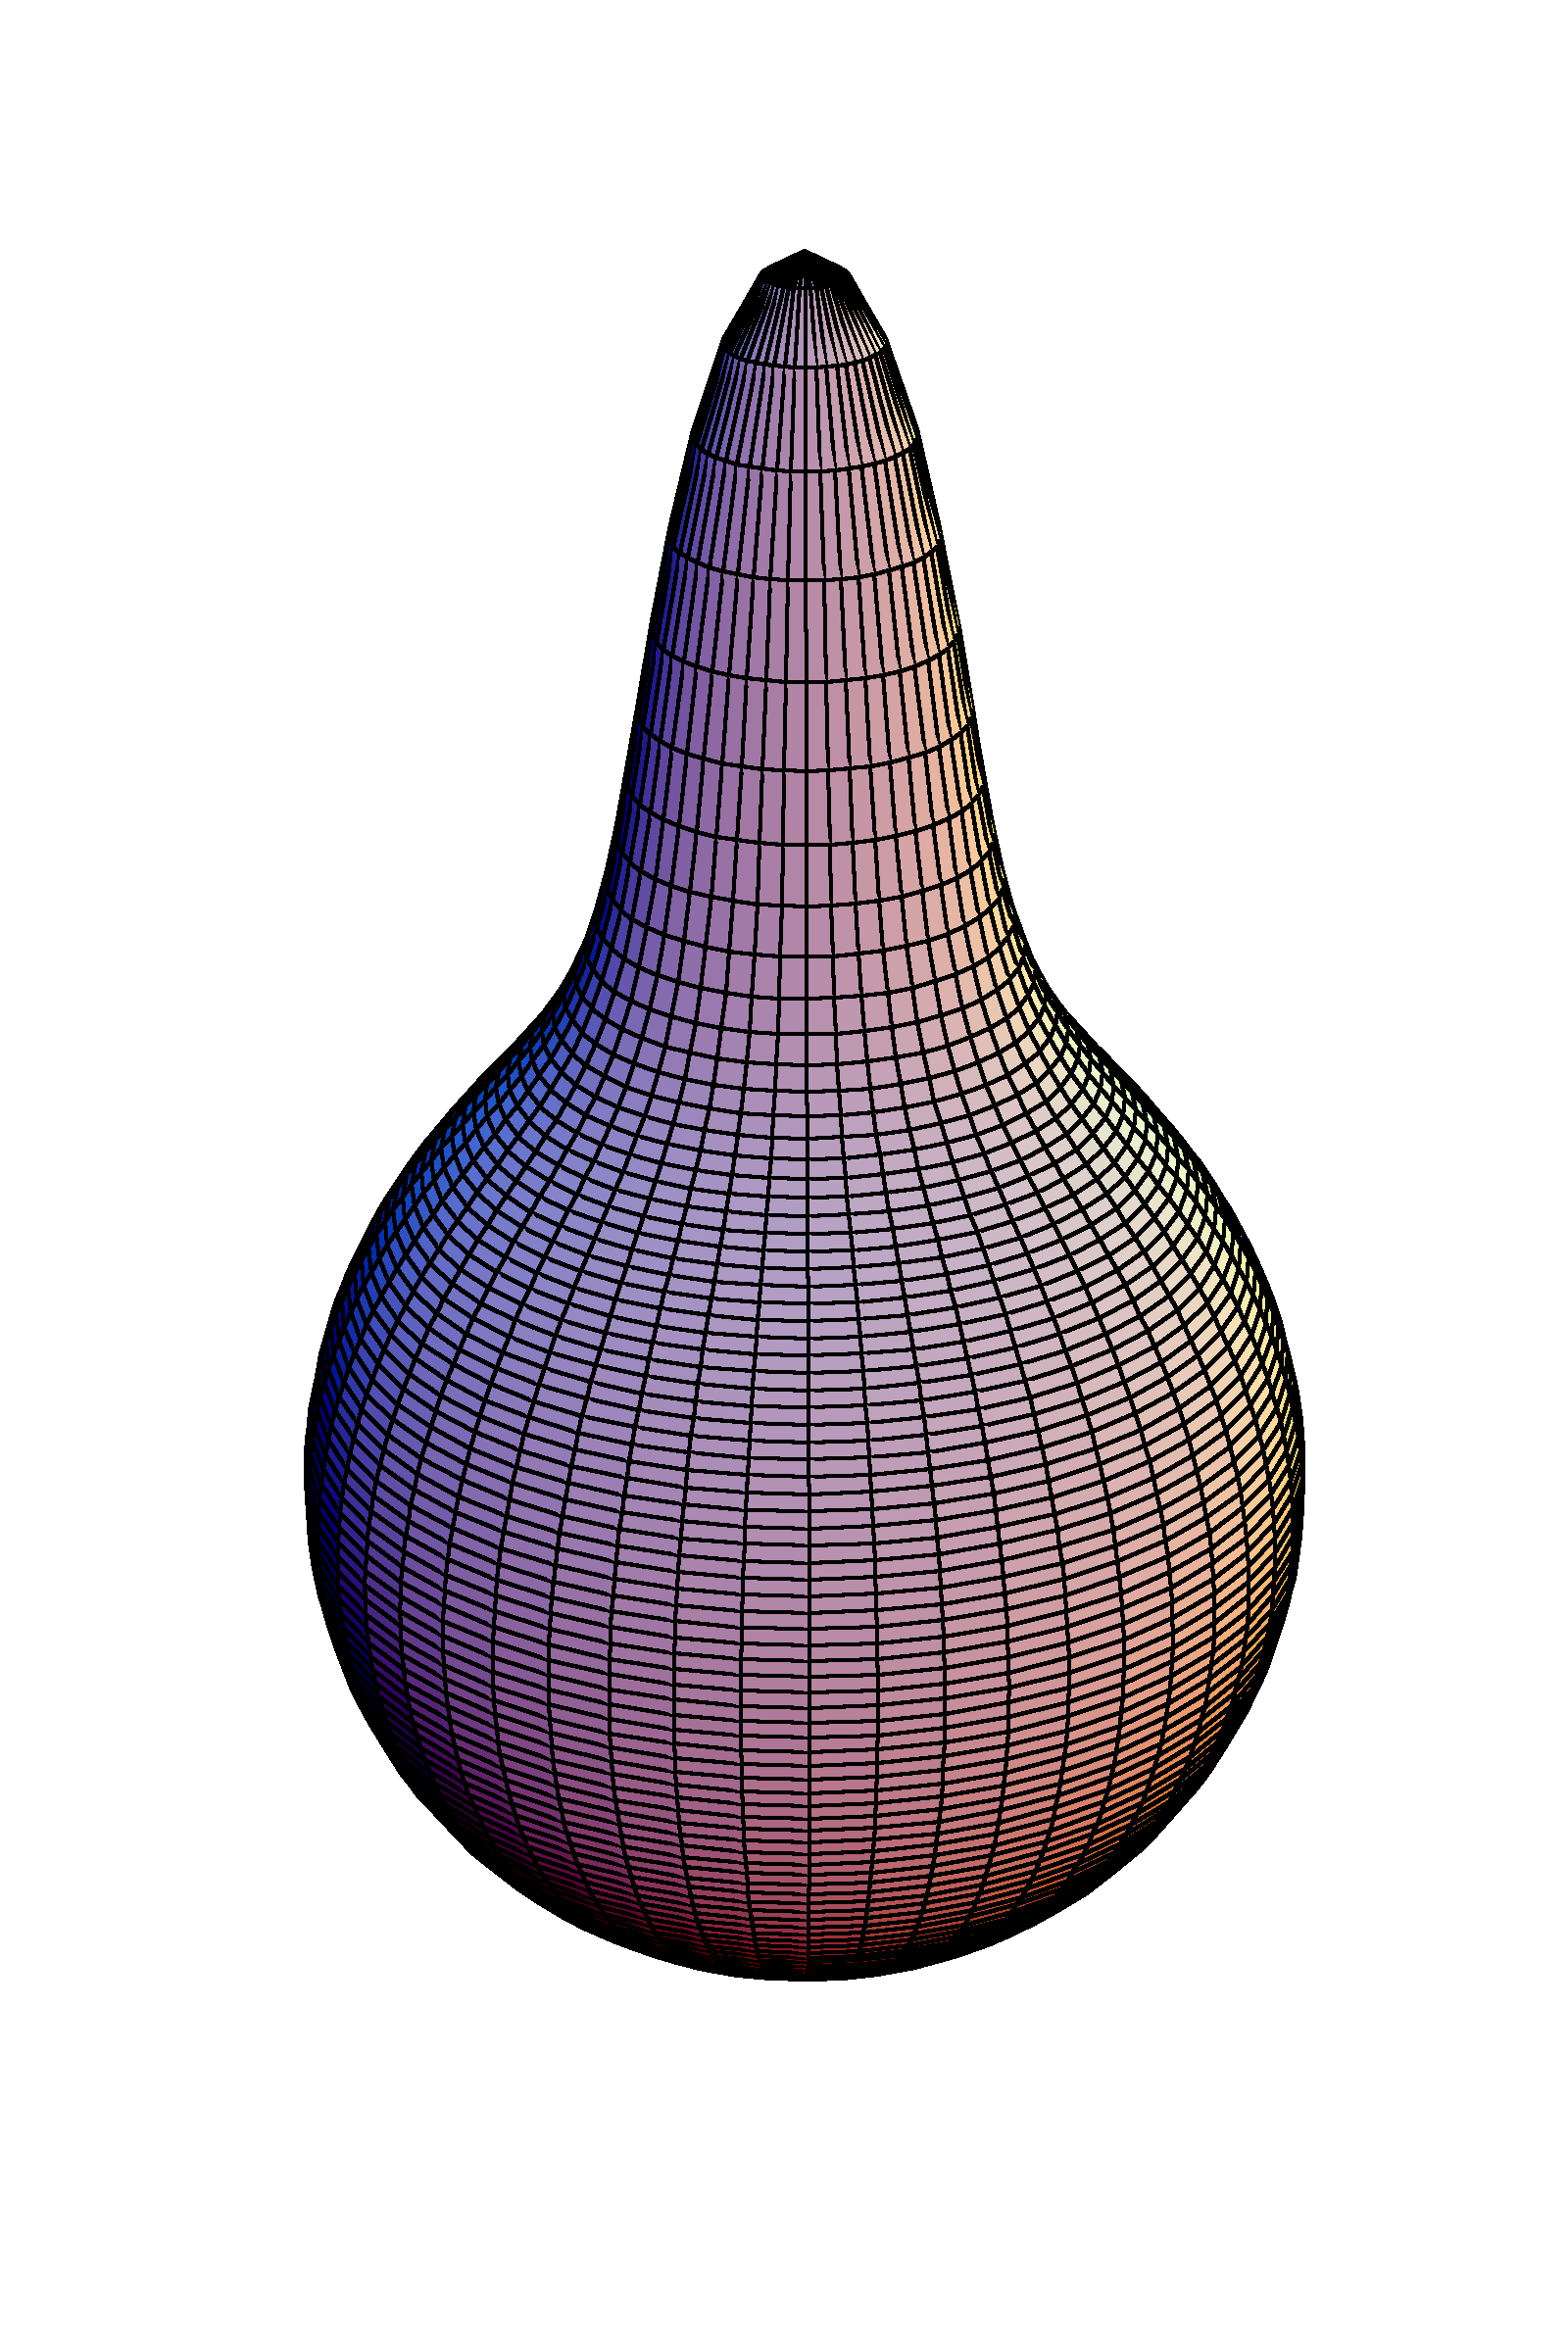
\includegraphics[width=0.5\textwidth]{images/p_080.png}}\hfill
   \subfigure[$h=0.85$]
     {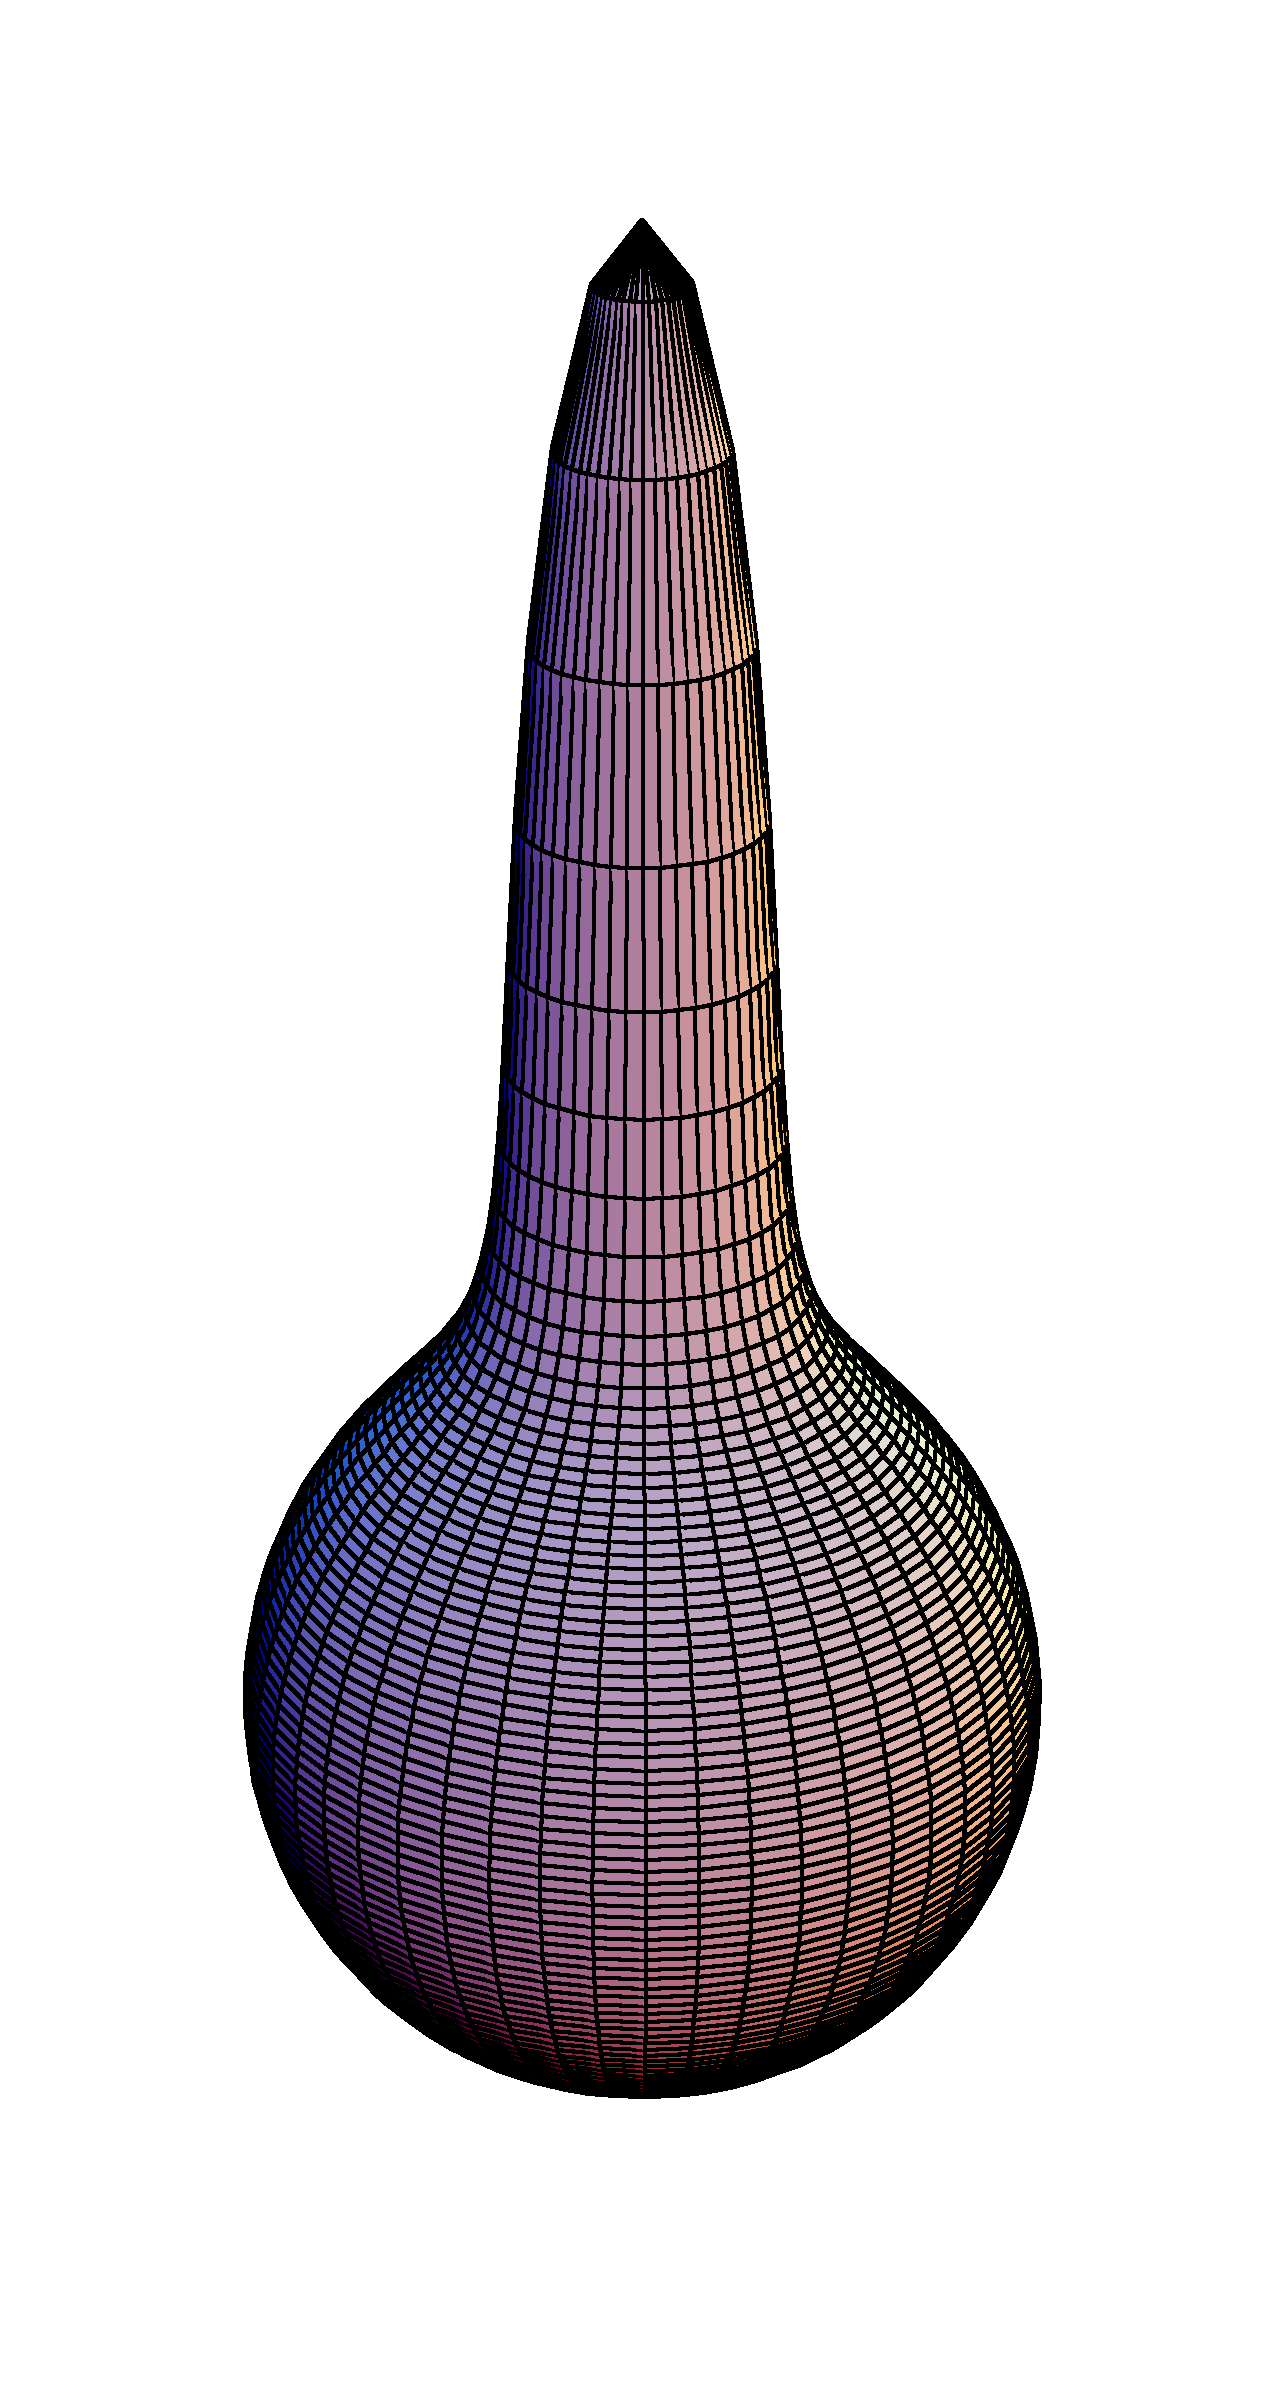
\includegraphics[width=0.5\textwidth]{images/p_085.png}}
  \caption{The Poisson kernel plotted as a spherical radial basis function on the sphere for different values of $h$.}
  \label{Basics:Figure:PoissonKernel2}
\end{figure}

\label{Basics:SphericalKernels}

\section{Discrete Cosine Transform}
\label{Basics:DiscreteCosineTransform}

The \emph{Discrete cosine transforms (DCTs)} are a class of real transforms closely related to the 
\emph{discrete Fourier transform (DFT)}. They exploit the fact that the 
input data is real and has even symmetry. The Fourier transform of a real-even 
function is real-even and $\im$ times the Fourier transform of a real-odd function is real-odd. 
Similar results hold for the DFT. Based on this fact, one can now define 
real transforms respecting the additional symmetry.
Due to the discrete sampling, we have an additional choice: The symmetry can be 
viewed relatively to a data point or to a point halfway between two data points. For our 
purposes we confine ourselves with introducing two variants.

We define the matrices
\begin{equation}
  \nonumber
  \V{C}_{N} := \paren{\cos \frac{j(2k+1) \pi}{2N}}_{j,k = 0}^{N-1}, \quad \V{D}_N := \diag\, \paren{\varepsilon_j^N}_{j = 0}^{N-1} \quad \paren{N \in \N}
\end{equation}
with $\varepsilon_0^N := \frac{1}{2}$ and $\varepsilon_j^N := 1$ for $j = 1,\ldots,N-1$.
The discrete cosine transforms DCT-II($N$) and DCT-III($N$) are then defined as follows:
\begin{equation}
  \label{Basics:DCT}
  \begin{split}
    \text{DCT-II($N$): } & \R^N \rightarrow \R^N,\ \V{\tilde{a}} := \V{C}_N\, \V{a},\\
    \text{DCT-III($N$): } & \R^N \rightarrow \R^N,\ \V{\tilde{b}} := \V{C}_N^{\transp} \V{D}_N\, \V{b}, 
  \end{split}  
\end{equation}
where $\V{a} := \paren{a_k}_{k=0}^{N-1} \in \R^N$ is the input vector and $\V{\tilde{a}} := 
\paren{\tilde{a}_j}_{j=0}^{N-1} \in \R^N$ is the output vector and similarly $\V{b}$ and $\V{\tilde{b}}$. 
The Chebyshev polynomials of the first kind $T_{k}$ are given by $\fun{T_{k}}{x} := \fun{\cos}{k \arccos x}$ 
and we obtain
\begin{equation}
  \label{Basics:DCT2}
  \begin{split}
    \tilde{a}_{j} & = \sum_{k = 0}^{N-1} a_{k} \cos \frac{j(2k+1)\pi}{2N} = \sum_{k = 0}^{N-1} a_{k} \fun{T_{j}}{\cos \frac{(2k+1) \pi}{2N}},\\
    \tilde{b}_{j} & = \sum_{k = 0}^{N-1} \varepsilon_k^N b_{k} \cos \frac{k(2j+1)\pi}{2N} = \sum_{k = 0}^{N-1} \varepsilon_k^N b_{k} \fun{T_{k}}{\cos \frac{(2j+1) \pi}{2N}}.
  \end{split}  
\end{equation}
The following lemma shows that the matrix $\V{C}_N$ is up to a scalar factor nearly orthogonal (for a proof see \cite{bata}).
\begin{lemma}
  \label{Basics:DCT3}
  Let $\V{C}_N$ and $\V{D}_N$ be defined as in \eqref{Basics:DCT}. Then we have
  $$ \V{C}_N\V{C}_N^{\transp}\V{D}_N = \V{C}_N^{\transp}\V{D}_N\V{C}_N = \frac{N}{2} \V{I}_{N}. $$
\end{lemma}
Therefore the DCT-II is the inverse of the DCT-III an vice versa up to a scaling factor.

\section{Fast Polynomial Multiplication}
\label{Basics:FastPolynomialMultiplication}
A polynomial $P \in \Pol_{K-1}$ is uniquely determined by its \emph{Chebyshev coefficients} 
$\paren{a_{k}}_{k = 0}^{K-1}$ with $\fun{P}{x} = \sum_{k=0}^{K-1} a_{k} \fun{T_{k}}{x}$. Given 
now a second polynomial $Q \in \Pol_{K}$, $K \in \NZ$ known in advance, we give a fast algorithm first described in \cite{postta97} for computing the 
Chebyshev coefficients of the polynomial product $R := P \: Q \in \Pol_{2K-1}$. The polynomial $R$ is uniquely determined 
by the products $f_{j} := \fun{P}{\cos \frac{(2j+1)\pi}{4K}} \fun{Q}{\cos \frac{(2j+1)\pi}{4K}}$ for $j = 0,\ldots,2K-1$ and 
by \eqref{Basics:DCT2} we obtain
\begin{eqnarray*}
  \paren{\fun{P}{\cos \frac{(2j+1)\pi}{4K}}}_{j=0}^{2K-1} = \V{C}_{2K}^{\transp} \paren{a_{k}}_{k=0}^{2K-1},\\
  \paren{\fun{Q}{\cos \frac{(2j+1)\pi}{4K}}}_{j=0}^{2K-1} = \V{C}_{2K}^{\transp} \paren{b_{k}}_{k=0}^{2K-1},
\end{eqnarray*}
where we set $a_{k} = 0$ for $k > K-1$ and $b_{k} = 0$ for $k > K$. This means that the evaluation 
of the polynomials $P$ and $Q$ can be performed using two DCT-IIIs of length $2K$ where we additionally have to 
compensate for the factors $\varepsilon_{k}^K$ introduced by the matrix $\V{D}_{2K}$.
Once calculated the products $f_{j}$ and taking into account that $\V{C}_{2K}^{-\transp} = \frac{2}{2K} \V{D}_{2K} \V{C}_{2K}$ 
by Lemma \ref{Basics:DCT3} we get
$$ \paren{c_{k}}_{k=0}^{2K-1} = \frac{2}{2K} \V{D}_{2K} \V{C}_{2K} \paren{f_{j}}_{j = 0}^{2K-1}.$$
This leads to the following algorithm:

\begin{algorithm}[ht]
  \caption{Fast polynomial multiplication in Chebyshev representation}
  \label{Basics:Algorithm:FastPolynomialMultiplication}    
  \begin{algorithmic}
    \STATE  Input:  $K = 2^t\; (t \in \N)$, $\paren{a_{k}}_{k = 0}^{K-1}$, $\paren{\fun{Q}{\cos \frac{(2j+1)\pi}{4K}}}_{0}^{"K-1}$
    \STATE
    \STATE Evaluate the polynomials at the Chebyshev nodes $\paren{\cos \frac{(2j+1)\pi}{4K}}_{j = 0}^{2K-1}$
      using two fast DCT-IIIs of length $2K$.
    \STATE 
    \FOR {$j=0,\ldots , 2K-1$} 
      \STATE $f_{j} := \fun{P}{\cos \frac{(2j+1)\pi}{4K}} \fun{Q}{\cos \frac{(2j+1)\pi}{4K}}$
    \ENDFOR
    \STATE
    \STATE Compute the Chebyshev coefficients $\paren{c_{k}}_{k=0}^{2K-1}$ using a fast DCT-II of length $2K$.
    \STATE
    \STATE Output: $\paren{c_{k}}_{k=0}^{2K-1}$
\end{algorithmic}
\end{algorithm}

\section{Fast Fourier Transform for Nonequispaced Knots}
\label{Basics:NFFT}

The \emph{nonequispaced fast Fourier transform (NFFT)} generalizes the well know \emph{fast Fourier transform (FFT)}. For the sake of simplicity, we restrict ourselves to the one-dimensional case on the torus $\mathbb{T} := \pset{x \in \R}{|}{-\frac{1}{2} \le x \le \frac{1}{2}}$. For fixed $M \in \N_{0}$ and $D \in \N$ we denote by $\mathcal{X} := \pset{x_{j} \in \mathbb{T}}{|}{j = 0,\ldots,D-1}$ a \emph{sampling set} of nodes from $\mathbb{T}$ and let $\mathcal{I}_{M} := \pset{k \in \Z}{|}{-\frac{M}{2} \le k \le \frac{M}{2}-1}$ be the index set of all possible \emph{frequencies}. The considered problem is the evaluation of a trigonometric polynomial 
$f: \mathbb{T} \rightarrow \C$ with
\begin{equation}
  \label{Basics:NFFT:f}
  \fun{f}{x} =: \sum_{k \in \mathcal{I}_{M}} \hat{f}_{k} \e^{- 2 \pi \im k x}
\end{equation}
on the sampling set $\mathcal{X}$. The algorithm is approximative with computational complexity $\bigo{M \log M + \fun{\log}{1/\varepsilon}D}$ where $\varepsilon$ is the desired accuracy. The technique used is to approximate the function $f$ in \eqref{Basics:NFFT:f} by a linear combination of shifted 1-periodic window functions $\varphi$ as
$$
  \fun{f}{x} \approx \fun{s}{x} := \sum_{l \in \mathcal{I}_{m}} g_{l} \fun{\tilde{\varphi}}{x - \frac{l}{m}}.
$$ 
The oversampling factor $\sigma > 1$ defines $m$ by $m := \sigma M$. An admissible window function $\tilde{\varphi}$ should be well localized in time and frequency and has
a uniform convergent Fourier series
$$
  \fun{\tilde{\varphi}}{x} = \sum_{k \in \Z} \fun{c_{k}}{\tilde{\varphi}} \e^{-2 \pi \im k x}
$$
with Fourier coefficients $\fun{c_{k}}{\tilde{\varphi}} \in \C$.
We refer the interested reader to \cite{duro93} and \cite{postta} for a detailed description of approximative algorithms for the NFFT and further related references.